\setcounter{ExampleCounter}{1}
Warren Buffett, in his regular letters to his partnerships, occasionally included a section titled ``The Joys of Compounding,'' which he called ``the pulse-quickening portion of our essay.''  In one such section in a letter from 1964, he wrote about the \emph{Mona Lisa}:
\marginnote{
\includegraphics[width=1.5in]{MonaLisa}}
\begin{quote}
Since the whole subject of compounding has such a crass ring to it, I will attempt to introduce a little class into the discussion by turning to the art world.  Francis I of France paid 4,000 ecus in 1540 for Leonardo da Vinci's \emph{Mona Lisa}.  On the off chance that a few of you have not kept track of the fluctuations of the ecu, 4,000 converted out to about 20,000.

If Francis had kept his feet on the ground and he (and his trustees) had been able to find a 6\% after-tax investment, the estate now would be worth something over \$1,000,000,000,000,000.00.  That's \$1 quadrillion or over 3,000 times the present national debt, all from 6\%.  I trust this will end all discussion in our household about any purchase of paintings qualifying as an investment.
\end{quote}

In a letter from the previous year, he concluded a similar example by saying
\begin{quote}
Such fanciful geometric progressions illustrate the value of either living a long time, or compounding your money at a decent rate.  I have nothing particularly helpful to say on the former point.
\end{quote}

Don't worry, though; he gives a less fanciful example, as well, showing a table like the one below, which shows the returns from a \$100,000 investment over 10, 20, and 30 years using different interest rates:
\begin{center}
\begin{tabular}{l c c c}
 & \textbf{4\%} & \textbf{8\%} & \textbf{12\%}\\
10 Years & \$48,024 & \$115,892 & \$210,584\\
20 Years & \$119,111 & \$366,094 & \$864,627\\
30 Years & \$224,337 & \$906,260 & \$2,895,970
\end{tabular}
\end{center}

A quick glance through this table should make the point clear: compound interest is a powerful force (there's an apocryphal quote often attributed to Albert Einstein in which he calls it the most powerful force in the universe).  Specifically, the power of compound interest comes from the length of time an investment is given to grow, and even small changes in the interest rate can have dramatic results over enough time.

By the way, although you won't find a bank account that offers interest rates anything close to the ones listed above, the long-term rate of return on the stock market is around 10\%, so these values are by no means fictional.

These examples show what happens with \emph{compound interest}, but we haven't yet discussed what that means.
\vfill

\begin{proc}{Simple and Compound Interest}
\paragraph{Simple Interest} Interest is calculated based on the principal alone (the interest rate describes what percentage of the principal is returned).\\

\paragraph{Compound Interest} The interest from one year (or month) is added to the principal, and the next year interest is calculated based on this combination of the principal and the past interest.
\end{proc}

\subsection{Simple Interest}
Suppose you take out a loan for \$500 at 10\% annual interest rate for 4 years.  Each year, (\$500)(0.1) = \$50 in interest accrues, so the total interest is 4 times this:
\[(\$500)(0.1)(4) = \$200\]
At the end of the 4 years, you'll have to pay back the principal, \$500, plus the interest, \$200, for a total of \$700, so a present value of \$500 grew to a future value of \$700.  Clearly, this growth depends on the interest rate and the amount of time involved.
\pagebreak

\text{}
\vfill

\begin{formula}{Simple Interest}
The interest, $I$, earned on a loan with principal $P$ at annual interest rate $r$ (expressed as a decimal) over a period of $t$ years is
\[I=Prt\]
This formula works with other time periods (months, for instance) as long as the interest rate is given in the same terms (so a monthly interest rate, for instance).

\paragraph{Future Value}
The future value ($F$) of this principal (or present value) $P$ is the sum of the principal and the interest:
\[F = P + Prt\]
\marginnote{Future value for simple interest}\[F = P(1+rt)\]
Other kinds of loans (like compound interest) will have different formulas for future value, but the principal is the same: this formula tells at what rate this pile of money will grow.
\end{formula}
\vfill

\paragraph{APR: Annual Percentage Rate} Note carefully that $t$ is measured in \textit{years}; this is consistent for almost all the financial formulas in this chapter.  This means that interest rates are given as \textit{annual} interest rates.  It's also possible to express loans in monthly terms.  To do so, the APR is divided into a monthly interest rate; for example, a 12\% APR would be 1\% monthly, a 6\% APR would be 0.5\% monthly, etc.
\vfill

\begin{example}{Simple Interest}
\marginnote{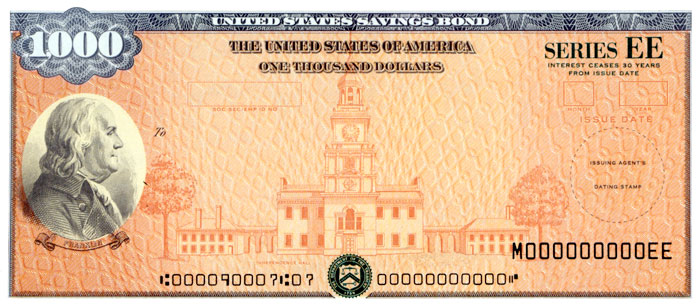
\includegraphics[scale=0.15]{TNote1}}
Treasury notes and savings bonds are issued by the federal government to cover its expenses and debt.
Suppose you obtain a \$1,000 Series EE savings bond with a 4\% annual rate and sell it 8 years later. How much interest will you earn?
\vspace{0.1in}

\sol
Use the simple interest formula above:
\begin{align*}
I &= Prt\\
&= (\$1000)(0.04)(8)\\
&= \boxed{\$320}
\end{align*}

You'll earn \$320 in interest, so at the end you'll have a total of \$1320.
\end{example}
\vfill

\begin{try}
You deposit \$3000 in a savings account at BB\&T Bank, earning 5\% interest.  Find the amount of interest earned and the total amount in the account after three years.
\end{try}

\vfill
When you're solving one of these problems, note carefully how the question is phrased.  Some may ask for the interest earned by an investment, while others may ask for the total value of the investment at the end, which is simply the principal plus the interest.

\vfill
\text{}
\pagebreak
\text{}
\vfill

\begin{example}{Future Value with Simple Interest}
If you deposit \$6200 at 6\%, what is the future value of the deposit at the end of 2.5 years?

\sol
Rather than calculating the interest first and adding that onto the principal, we can use the future value formula to do both steps at once:
\begin{align*}
F &= P(1+rt)\\
&= \$6200(1+(0.06)(2.5))\\
&= \boxed{\$7130}
\end{align*}
\end{example}
\vfill

\begin{try}
What is the future value of a \$2400 at 7\% simple interest at the end of three years?
\end{try}
\vfill

We can also turn the problem around: if we know how much we want an investment to be worth in the future, we can use a little algebra to solve for the present value, or the principal.
\vfill

\begin{example}{Present Value with Simple Interest}
You'd like to buy a \$12,000 car in 18 months, and your bank is offering 6\% simple interest.  How much should you deposit now in order to have a final balance of \$12,000?

\solline
\marginnote{
\includegraphics[scale=0.15]{VWVan1}}
We can use the same future value formula as in the previous example, but now the future value is given, and the present value is the unknown part:
\begin{align*}
F &= P(1+rt)\\
\$12,000 &= P(1+(0.06)(1.5))\\
\end{align*}

Note that $t=1.5$, since $t$ is measured in years, and 18 months is one-and-a-half years.\\

Now solve this for $P$ to find the amount that you need to deposit today:
\begin{align*}
\$12,000 &= P(1.09)\\
\dfrac{\$12,000}{1.09} &= P\\
\boxed{\$11,009.17} &= P
\end{align*}
You'll need to deposit \$11,009.17 today in order to have \$12,000 in the account in 18 months.
\end{example}
\vfill

\begin{try}
How much do you need to deposit today in an account earning 3\% simple interest to have \$800 in 36 months?
\end{try}
\vfill
\pagebreak

\subsection{Compound Interest}
With simple interest, we assumed that we pocketed the interest when we received it.  If, on the other hand, we added that interest to the account, we could earn interest on that interest in the future, making the balance grow a little bit faster.  This reinvestment of interest is called \textbf{compounding}.\\

Suppose we deposit \$5000 for 5 years in an account offering an 8\% APR, with interest compounded yearly.  How much will be in the account at the end?

At the end of each year, 8\% of the balance at that point will be added to the account, and the balance will grow.  The following table shows on a year-to-year basis the total dollar amount in the account at the end of each year and the interest that accrues that year.
\begin{center}
\begin{tabular}{| c | p{1in} | p{1.52in} | p{1.5in} |}
\hline
{\small Year} & {\small Starting Balance} & {\small Interest Earned} & {\small Final Balance}\\
\hline
1 & \$5000 & $\$5000 \times 0.08 = \$400$ & $\$5000 + \$400 = \$5400$\\
\hline
2 & \$5400 & $\$5400 \times 0.08 = \$432$ & $\$5400 + \$432 = \$5832$\\
\hline
3 & \$5832 & $\$5832 \times 0.08 = \$467$ & $\$5832 + \$467 = \$6299$\\
\hline
4 & \$6299 & $\$6299 \times 0.08 = \$504$ & $\$6299 + \$504 = \$6803$\\
\hline
5 & \$6803 & $\$6803 \times 0.08 = \$544$ & $\$6803 + \$544 = \$7347$\\
\hline
\end{tabular}
\end{center}
The total amount in the account at the end of the fifth year is \$7347, which is \$347 more than we would have earned using simple interest.

Notice that each year, the amount of interest that we earned grew, making the account grow faster and faster.  This is the advantage of compounding, and over long periods of time it can lead to very dramatic results.\\

Following this example, we can derive a formula to take care of the calculation for us so that we don't have to build a table like this every time.  At the end of the first year, the balance had grown to \[\$5000+(\$5000)(0.08) = \$5000(1+0.08).\]  Following the pattern, each year the balance is multiplied by $(1+0.08)$, so at the end of the second year, the balance grew to 
\[\$5000(1+0.08)(1+0.08) = \$5000(1+0.08)^2.\]  At the end of the third year, then, the account would hold \[\$5000(1+0.08)^3\] and so on.  

After $t$ years, the amount in an account with an interest rate of $r$, compounded once per year, will be\marginnote{Future value for interest compounded yearly} \[F=P(1+r)^t\]

\paragraph{What if interest isn't compounded yearly?} The formula we just derived assumes that interest is compounded---or added to the account---at the end of each year.  However, this doesn't have to be the case; interest could be compounded twice a year (semiannually), four times a year (quarterly), monthly, weekly, or even daily.  \marginnote{\begin{tabular}{r | l}
{\small Compounded} & $n$\\
\hline
{\small Annually} & 1\\
{\small Semiannually} & 2\\
{\small Quarterly} & 4\\
{\small Monthly} & 12\\
{\small Weekly} & 52\\
{\small Daily} & 365\footnotemark
\end{tabular}}\footnotetext{Before calculators were commonplace, some calculations used $n=360$ for daily compounding to make the arithmetic simpler} keep track of how often interest is compounded, we define $n$ as the \textbf{number of times per year that interest is compounded}, regardless of how many years the account grows.

Now if we split the year into $n$ segments, the interest rate will be divided up as well, so each segment will earn an interest rate of $\frac{r}{n}$, so that will replace $r$ in the compound interest formula.  Also, rather than having the interest accrue $t$ times, it will accrue $n$ times each year for $t$ years, or a total of $nt$ times, so that will replace $t$ in the compound interest formula.

All of this brings us to the complete formula for the future value of an investment with compound interest.
\begin{formula}{Compound Interest}
The future value $F$ of a principal amount $P$ with an annual interest rate $r$ (expressed as a decimal) compounded $n$ times per year for $t$ years is
\[F=P\left(1+\dfrac{r}{n}\right)^{nt}\]
Notice that if interest is compounded yearly, $n=1$, and the formula becomes the one we derived after the example above.
\end{formula}
\pagebreak

\begin{example}{Certificate of Deposit}
A certificate of deposit (CD) is an account that many banks offer that often comes with a higher interest rate, but the investment cannot be touched for a specified length of time.  Suppose you deposit \$3000 in a CD earning 6\% interest compounded monthly.  How much will you be able to withdraw at the end of 20 years?

\sol
List the pieces of the formula that are given:
\begin{center}
\begin{tabular}{l l}
$P$ & \$3000\\
$r$ & 0.06\\
$n$ & 12\\
$t$ & 20
\end{tabular}
\end{center}
So at the end of the 20 years, the account will hold 
\[F = 3000\left(1+\dfrac{0.06}{12}\right)^{(12)(20)} = \boxed{\$9930.61}\]

\solline
Now compare this to the amount you would earn from simple interest.
\begin{center}
\begin{tabular}{l | r | r}
Years & Simple Interest & Compound Interest\\
\hline
5 & \$3900 & \$4046.55\\
10 & \$4800 & \$5458.19\\
15 & \$5700 & \$7362.28\\
20 & \$6600 & \$9930.61\\
25 & \$7500 & \$13,394.91\\
30 & \$8400 & \$18,067.73\\
35 & \$9300 & \$24,370.65
\end{tabular}
\vspace{0.2in}

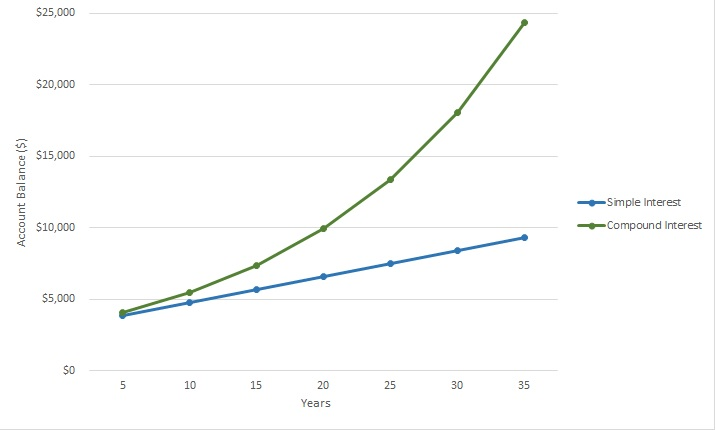
\includegraphics[scale=0.65]{SimpleCompoundGraph}
\end{center}
This illustrates the difference between the linear growth offered by simple interest and the exponential growth offered by compound interest.  Over a long period of time, compounding makes a huge difference.
\end{example}

\begin{try}
If you deposit \$700 at 5\% interest compounded monthly, how much will the account hold in 13 years?
\end{try}
\pagebreak
\text{}
\vfill

\begin{proc}{Using Your Calculator: Exponents}
\begin{tabular}{c l}
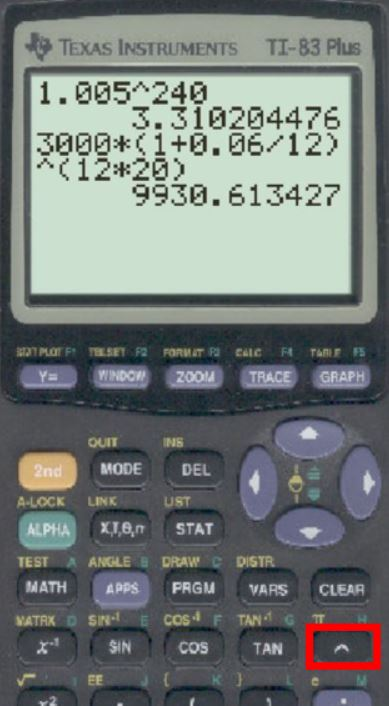
\includegraphics[scale=0.35]{Calculator1} & \parbox[b]{3in}{To evaluate an exponent like $1.005^{240}$ we use the exponent key like the one shown, or possibly $\boxed{y^x}$ or $\boxed{x^y}$ on some calculators.\\

Be careful when evaluating these often-complicated financial formulas; it's usually safer to evaluate them in pieces, like in the first line, where we began by calculating $1+0.06/12 = 1.005$ and $(12)(20)=240$, and then using the exponent key.  If you want to evaluate the entire formula in one step, be careful to use parentheses to do each operation in the proper order, as shown in the second line.\\

Also, be very careful with rounding; keep at least three significant digits (digits after leading zeros) from one calculation to the next, or use the calculator storage function.}
\end{tabular}
\end{proc}
\vfill

Just as we did with simple interest, we can also solve for present value with compound interest if we know what we want the future value to be.
\vfill

\begin{example}{Saving for College}
You know that you will need \$40,000 for your child's education in 18 years.  If your account earns 4\% compounded quarterly, how much would you need to deposit now to reach your goal?

\sol
List the pieces of the formula that are given:
\begin{center}
\begin{tabular}{l l}
$F$ & \$40,000\\
$r$ & 0.04\\
$n$ & 4\\
$t$ & 18
\end{tabular}
\end{center}
In this example, $F$ is given and $P$ is unknown:
\[40,000 = P\left(1+\dfrac{0.04}{4}\right)^{(4)(18)}\]
Solve for $P$:
\begin{align*}
P &= \dfrac{40,000}{\left(1+\dfrac{0.04}{4}\right)^{(4)(18)}}\\
&= \boxed{\$19,539.84}
\end{align*}
\end{example}
\vfill

\begin{try}
If you want to have \$26,000 in a college fund in 12 years, and you find an account earning 5\% compounded daily, how much should you deposit now?
\end{try}
\vfill
\text{}
\vfill
\pagebreak
\text{}
\vfill

\begin{proc}{Using Your Calculator: Avoid Rounding If You Can}
In many cases, you can avoid rounding to make your answers more precise based on how you use your calculator.  For example, to calculate something like
\[F = 1000\left(1+\dfrac{0.05}{12}\right)^{(12)(30)}\] start from the inside and work outward.  We can quickly calculate (maybe even mentally) that $(12)(30) = 360$, and now we can use the calculator:
\begin{center}
\begin{tabular}{c | c}
\textbf{Type This} & \textbf{Calculator Shows}\\
\hline
0.05 $\boxed{\div}$ 12 $\boxed{=}$ & 0.00416666666667\\
$\boxed{+}$ 1 $\boxed{=}$ & 1.00416666666667\\
$\boxed{y^x}$ 360 $\boxed{=}$ & 4.46774431400613\\
$\boxed{\times}$ 1000 $\boxed{=}$ & 4467.74431400613
\end{tabular}
\end{center}
\end{proc}
\vfill

\begin{example}{Don't Round Too Much}
To see why not over-rounding is so important, suppose you were investing \$1000 at 5\% compounded monthly for 30 years.
\begin{center}
\begin{tabular}{l l}
$P$ & \$3000\\
$r$ & 0.06\\
$n$ & 12\\
$t$ & 20
\end{tabular}
\end{center}
To use the formula, we'll need $\frac{r}{n}$, which is 0.0041666666666$\ldots$\\

Notice the effect of rounding this to different values:
\begin{center}
\begin{tabular}{l l l}
$r/n$ rounded: & Gives $F$ to be: & Error\\
\hline
No rounding & \$4467.74 & \\
0.0041667 & \$4467.80 & \$0.06\\
0.004167 & \$4468.28 & \$0.54\\
0.00417 & \$4473.09 & \$5.35\\
0.0042 & \$4521.45 & \$53.71\\
0.004 & \$4208.59 & \$259.15
\end{tabular}
\end{center}
Notice that the error grew by \textit{about} a factor of 10 each time, which is not unusual, considering that we rounded off a digit each time. \\

For our purposes, the answer we got by rounding to 0.004167 (four significant digits) is good enough - as long as we're not working in a bank, a rounding error of \$0.54 is fine for us.
\end{example}
\vfill
\text{}
\vfill
\pagebreak

\subsection{Comparing Interest Rates}
\begin{example}{Comparing Banks}
\marginnote{
\includegraphics[scale=0.1]{Lottery1}}
You have just won \$500 in the Daily Pick 3 lottery and you decide to deposit your winnings in the bank.  You check with two different banks, which offer different options.  M\&T Bank offers a 4.25\% interest rate compounded daily, while SunTrust offers 4.3\% compounded annually.  Which bank should you choose?

\solline
To compare the two banks, simply choose an arbitrary amount of time and calculate how much each account would hold at the end of that time; whichever is higher is the one you'll choose.  Let's pick a year as our length of time, just for simplicity.  The table below shows the results of calculating the future value of your \$500 at the end of a year with each bank.
\begin{center}
\begin{tabular}{c c}
M\&T & SunTrust\\
\hline
& \\
\$521.71 & \$521.50
\end{tabular}
\end{center}
Even though the difference is relatively small, you'll choose the first account, since over time the difference may grow to something more significant.
\end{example}
\vfill

That example illustrates an important point: you'll often find different loans or accounts expressed in different terms, perhaps with different interest rates and compounding periods.  In that case, you'll want to find some way to put them all on equal footing to compare them; like we did in that example, you can often do a quick calculation to see which will earn more in some arbitrary amount of time.

Banks will often take advantage of the financial illiteracy of their clients to present a loan in terms that will subtly benefit them.  The major goal of this chapter is to turn you into a financially literate, savvy consumer.
\vfill

\begin{proc}{Sidenote: Different Interest Rates}
There are different terms you may find if you go looking for interest rates, so we'll mention a few of them here:

\paragraph{Nominal Interest Rate} The \textit{nominal interest rate} is the interest rate that is stated, such as a 3\% annual rate on a bond or a 1.7\% monthly rate on a credit card.

\paragraph{Annual Percentage Rate (APR)} This is the annual nominal rate.  So for instance, the 1.7\% nominal monthly rate would correspond to a $1.7\% \times 12 = 20.4\%$ APR.

\paragraph{Effective Interest Rate (APY)} This is the real interest rate.  The \textit{effective rate}, also called the \textit{annual percentage yield (APY)} or the \textit{effective annual yield}, takes the compounding period into account.  This is done by calculating the simple interest rate that would lead to the same growth as that of the compound interest that is offered.

\paragraph{APR vs APY} Since APY takes the effect of compounding into account and APR does not, the APY will be slightly higher than the APR for a typical account.  Because of this, banks typically report the APR for debt-related accounts like credit cards and mortgages, and they report the APY for interest-bearing accounts like CDs and money market accounts.
\end{proc}
\vfill
\text{}
\vfill
\pagebreak

\subsection{Continuously Compounded Interest}
We've seen that compound interest makes money grow faster than simple interest does, but we can go even further: if someone offered you an investment compounded monthly and one compounded daily (with everything else equal), which would you choose?  You would be wise to choose the one that is compounded daily, because the more frequently that interest is compounded, the longer that interest that is added has to grow.  In other words, the interest that is added after one day has more time to grow than if it had to wait until the end of the month to be added.

The question is this: is there a limit to this growth?  Could we compound more and more often and see our money grow infinitely?  To answer this, suppose we deposit \$1 for one year into an account with a fixed interest rate---we'll use 100\% to illustrate, even though you'll almost certainly never encounter such an interest rate in real life---and we'll see what happens as we increase $n$, the frequency with which the interest is compounded:
\begin{center}
\begin{tabular}{r r}
$n$ & \hspace{0.5in} $1\left(1+\dfrac{1}{n}\right)^n$\\
& \\
\hline
& \\
1 & 2.0000000$\ldots$\\
5 & 2.4883200$\ldots$\\
10 & 2.5937424$\ldots$\\
50 & 2.6915880$\ldots$\\
100 & 2.7048138$\ldots$\\
1000 & 2.7169239$\ldots$\\
10,000 & 2.7181459$\ldots$\\
100,000 & 2.7182682$\ldots$\\
1,000,000 & 2.7182804$\ldots$\\
10,000,000 & 2.7182816$\ldots$\\
\end{tabular}
\end{center}

Notice that as we compound more and more frequently, we start to approach a limit.  This limit happens to be a very important number, so important that the letter $e$ is reserved for it.  It forms the basis of exponential growth, which has applications in every field of applied mathematics.\\

For a general interest rate $r$, $\left(1+\dfrac{r}{n}\right)^{nt}$ approaches $e^{rt}$ as the compounding increases.  This is what we call \textit{continously compounded interest}.

\begin{formula}{Continuous Compound Interest}
A present value $P$ will grow to a future value of $F$ under continuous compounding at an interest rate of $r$ according to:
\[F = Pe^{rt}\]
\end{formula}

\begin{proc}{Using Your Calculator: $e$}
\begin{tabular}{c l}
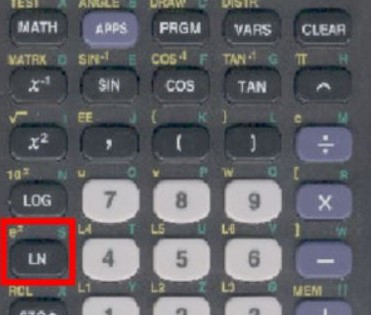
\includegraphics[scale=0.35]{CalculatorECropped} & \parbox[b]{3in}{Your calculator will most likely have a button for $e$, but depending on what kind of calculator you have, it may look different.\\

Here, the model shown has $e^x$ as the 2nd function of the button marked $\boxed{\textrm{LN}}$\ , so to calculate $e^{0.5}$, for instance, you would press $\boxed{\textrm{2nd}}$\ , then $\boxed{\textrm{LN}}$\ , then enter 0.5, and you should get 1.648721271.\\

On some scientific calculators, you may need to enter 0.5 and then press the $\boxed{e^x}$ key to get the same result.}
\end{tabular}
\end{proc}
\pagebreak

\begin{example}{Continuous Compound Interest: Future Value}
If you deposit \$4500 in an account paying 3.2\% interest compounded continuously, how much will the account hold after 36 months?

\sol
Use the continuous compound formula:
\begin{align*}
F &= Pe^{rt}\\
&= \$4500e^{(0.032)(3)}\\
&= \boxed{\$4953.42}
\end{align*}
\end{example}

\begin{try}
If you deposit \$13,000 in an account paying 2.8\% interest compounded continuously, how much will the account hold after 3 years?
\end{try}
\vfill

Once again, we can also turn the problem around and solve for the present value.
\vfill

\begin{example}{Continuous Compound Interest: Present Value}
How much will you need to deposit today at 5.3\% compounded continuously in order to have \$6300 in 4 years?

\sol
Just like before, we'll use the same formula, but now $F$ is known and $P$ is the unknown part.
\begin{align*}
F &= Pe^{rt}\\
\$6300 &= Pe^{(0.053)(4)}\\
\$6300 &= P(1.2361)\\
\dfrac{\$6300}{1.2361} &= P\\
\boxed{\$5096.48} &= P
\end{align*}
\end{example}
\vfill

\begin{try}
How much will you need to deposit today at 3.6\% compounded continuously in order to have \$1200 in 5 years?
\end{try}
\vfill
\text{}
\vfill
\pagebreak

\begin{example}{Comparing Different Compounding Periods}
You have \$7000 to invest for 5 years.  Find how much you'll have at the end of the 5 years if you earn 4\% compounded
\begin{enumerate}[(a)]
\item annually
\item monthly
\item daily
\item continuously
\end{enumerate}

\sol
The first three all use the same formula, and all that changes is $n$:
\begin{enumerate}[(a)]
\item Compounded annually:
\begin{align*}
F &= P\left(1+\dfrac{r}{n}\right)^{nt}\\
&= 7000\left(1+\dfrac{0.04}{1}\right)^{(1)(5)}\\
&= \$8516.57
\end{align*}

\item Compounded monthly:
\begin{align*}
F &= P\left(1+\dfrac{r}{n}\right)^{nt}\\
&= 7000\left(1+\dfrac{0.04}{12}\right)^{(12)(5)}\\
&= \$8546.98
\end{align*}

\item Compounded daily:
\begin{align*}
F &= P\left(1+\dfrac{r}{n}\right)^{nt}\\
&= 7000\left(1+\dfrac{0.04}{365}\right)^{(365)(5)}\\
&= \$8549.73
\end{align*}

\item Compounded continuously: \textbf{note the different formula}
\begin{align*}
F &= Pe^{rt}\\
&= 7000e^{(0.04)(5)}\\
&= \$8549.82
\end{align*}
\end{enumerate}
\end{example}

\begin{try}
If you deposit \$300, how much will you have in 7 years if you receive 3.5\% interest compounded
\begin{enumerate}[(a)]
\item quarterly?
\item monthly?
\item weekly?
\item continuously?
\end{enumerate}
\end{try}

Notice how the future value increases as interest is compounded more and more frequently.  The limit, of course, is the continuous case.
\pagebreak

\paragraph{Doubling Time} One common measure used to quickly compare investments is to determine how long it will take to double an investment.  The shorter the doubling time, the better the investment.

\begin{proc}{Solving Exponential Equations}
To solve an exponential equation, we use logarithms.  For exponential equations, we'll use the \textit{natural logarithm}, $\ln$.
\[\textrm{If } e^x = y, \textrm{ then } x = \ln y\]
\end{proc}

For more on solving equations involving exponents, see the algebra review chapter at the end of the book.

\begin{example}{Doubling Time}
Find the time required to double an investment at 6\% interest compounded continuously.\\

\sol
We could again pick an arbitrary amount for $P$, and let $F$ be double that.  Instead, though, we'll simply replace $F$ with $2P$, and solve the formula for $t$:
\begin{align*}
F &= Pe^{rt}\\
2P &= Pe^{0.06t}\\
\marginnote{note the change from exponential form to logarithmic form here}
2 &= e^{0.06t}\\
\ln 2 &= 0.06t\\
\dfrac{\ln 2}{0.06} &= t\\
\boxed{11.55} &= t
\end{align*}
Thus the investment will take approximately 11.5 years to double.
\end{example}

\begin{try}
How long will it take an investment to double at 5\% compounded continuously?
\end{try}

\begin{proc}{Doubling Time: the Rule of 72}
A quick way\marginnote{For continuous compounding, the \emph{Rule of 69.3} is more precise, but 72 is an easier number to use for mental calculations, and other compounding terms will give results closer to the Rule of 72 than continuous compounding does.} to roughly approximate doubling time is to divide 72 by the percent interest rate (i.e. not the decimal form, but 100 times that)
\[\textrm{Doubling Time } \approx \dfrac{72}{R}\]
where $R = 100r$.
\end{proc}

So for example, with an interest rate of 6\%, as in the last example, we could estimate the doubling time by dividing 72 by 6:
\[\dfrac{72}{6} = 12\]
Even though this isn't as precise as the calculation in the example, notice how much simpler it was, and knowing that our investment will double in about 12 years is just as valuable as knowing it will be precisely 11.55 years.
\pagebreak

\subsection{Using The TVM Solver}
If you have a TI-83 or TI-84 graphing calculator (or a similar model), you have a built-in application that can solve questions involving compound interest without using the formulas in this section.

Although we'll show you how to use it here, and it is possible to answer the homework questions using it, you should make sure that you can solve the problems using the formulas, just to stretch your mathematical muscles.

To begin, find the button marked $\boxed{\textrm{APPS}}$\ .  When you press that, you should have the option to select the Finance app, and when you press Enter twice, you'll enter the TVM (Time Value of Money) solver.  You should then see a screen like the following one.

\begin{center}
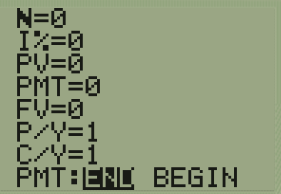
\includegraphics[width=2in]{TVMintro}
\end{center}

It's a good idea to zero out all the values at first (other than P/Y and C/Y), to make sure that you don't mistakenly use a value from another problem.

Let's go through the entries one at a time:
\begin{itemize}
\item N: the total number of compounding periods.  This means, for instance, that if interest is compounded monthly for 8 years, N would be $(12)(8) = 96$.  You could either calculate this separately, or simply type \texttt{12*8} in the space for N.  Just remember that since there's no entry for $t$, this value N is equal to $nt$ from our previous work.
\item I\%: the interest rate \textbf{as a percentage}, not a decimal.  For instance, if the interest rate is 4.5\%, simply enter 4.5 for I\%.
\item PV: the present value.  Note that the TVM solver uses the sign to indicate which direction the money is moving; cash outflow is negative, and income is positive.  If you deposit \$1000, for instance, you can enter -1000 for the present value, and the corresponding future value will be positive, since you'll recoup your investment.
\item PMT: a recurring payment.  This will come into play in the next section, but there's no need to use it for now; you can leave it as 0.
\item FV: the future value.  Again, the sign of this number will indicate which direction the money is moving.
\item P/Y: payments per year.  This too relates to the recurring payments that we'll encounter in the next section, but notice that it will always be the same as the next entry.
\item C/Y: compounding periods per year.  This is the familiar $n$ we've been using in the compound interest formula.
\end{itemize}

You can ignore the option at the end; that toggles between payments made at the beginning and end of the payment period, but we're not getting that involved.\\

The way to use this application is to enter all the information that's given, then use the SOLVE option (one of the alternate functions of the $\boxed{\textrm{ENTER}}$ key) to find the one that is unknown.  We'll illustrate with an example.
\pagebreak

\begin{example}{Using the TVM Solver}
Use the TVM solver on your calculator to find the present value needed if we want a future value of \$5000 in 6 years, if we can earn 4.3\% interest compounded monthly.

\sol
Open the TVM solver and try entering all the information that is given.  When you're done, you should see the following:
\begin{center}
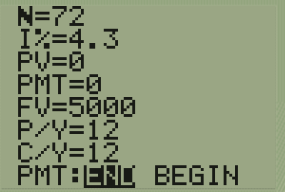
\includegraphics[width=2in]{TVMexample1}
\end{center}

Now, move the cursor to hover over the 0 next to PV=.  To access the SOLVE function on the $\boxed{\textrm{ENTER}}$ key, first press the $\boxed{\textrm{ALPHA}}$ key near the upper left corner of the keypad, then press the $\boxed{\textrm{ENTER}}$ key.

When you do, you should see the following:
\begin{center}
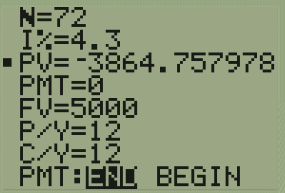
\includegraphics[width=2in]{TVMexample2}
\end{center}

Notice that the present value is given as a negative number, which indicates that if you want to receive (positive) \$5000 in the future, you need to deposit (negative) \$3864.76 now.
\end{example}

You can also use the TVM solver, for instance, to calculate the necessary interest rate if you enter both a present value and a future value.\\

Of course, there's no magic to this application; it's simply using the formulas you have already been using, and you could solve any of these problems the long way.  But it certainly is convenient to save yourself some typing.

\paragraph{Sidenote: Continuous Compounding} In case you're wondering how to handle continuous compounding, it turns out that it can be done, but it's a bit harder.

Since continuous compounding is essentially like interest compounding every instant, if we enter a huge number for C/Y, we can simulate this.  In practice, something like 1 million works well enough.  Then, let N be the number of years (so pretending that $n=1$) and let P/Y be 1, and the result will be as close as we need it to be.
\vfill
\pagebreak

\subsection{Using Excel}
Although there are some built-in formulas in Excel to calculate things like future value, it turns out that it's just as easy to create the formulas yourself and build a simple compound interest calculator.

To begin, open Microsoft Excel and enter the following labels in the first column of a worksheet:
\begin{center}
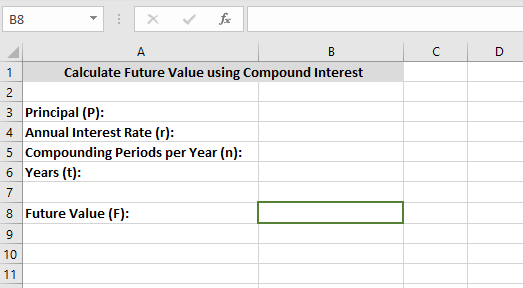
\includegraphics[width=3.5in]{ExcelExample1}
\end{center}

Notice that the highlighted cell (B8, since it is in column B and row 8) is where we want to find our answer.  We'll place the inputs in cells B3-B6:
\begin{center}
\begin{tabular}{c c}
\textbf{Value} & \textbf{Cell}\\
\hline
$P$ & B3\\
$r$ & B4\\
$n$ & B5\\
$t$ & B6
\end{tabular}
\end{center}

Thus, since the formula for $F$ is 
\[F = P\left(1+\dfrac{r}{n}\right)^{nt}\]
we can simply replace each variable with the corresponding cell in the formula we type into cell B8:
\begin{center}
Type ``\texttt{=B3*(1+B4/B5)}$\wedge$\texttt{(B5*B6)}'' into the formula box for cell B8.
\end{center}
Notice that we need to explicitly include a multiplication symbol when we want to multiply two values.
\begin{center}
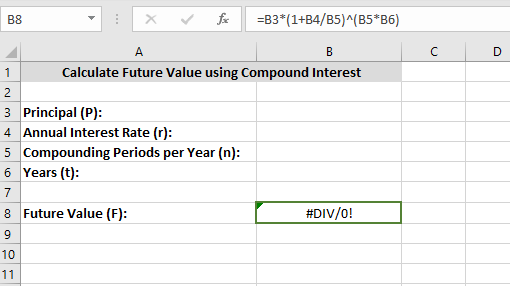
\includegraphics[width=3.5in]{ExcelExample2}
\end{center}

Notice that the result is an error at first, since we haven't filled in the other values, so the formula is forced to divide by 0, which of course isn't allowed.
\vfill
\pagebreak

Say, for instance, we want to find the future value of a \$2000 investment at 3\% for 5 years, compounded monthly.  Note that this time we'll use 0.03 for the interest rate, since the formula assumes $r$ is in decimal form.
\begin{center}
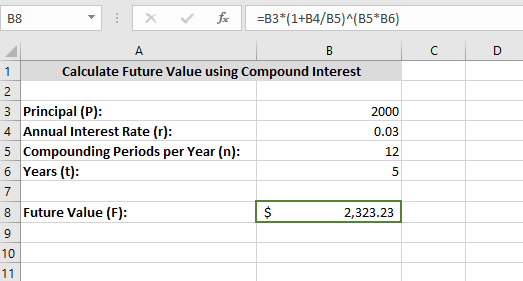
\includegraphics[width=3.5in]{ExcelExample3}
\end{center}

Notice that the output can be nicely formatted as a dollar amount by opening the Format Cells option after right-clicking on the cell.\\

There are many more ways to use Excel as a financial tool, but to calculate the result of compound interest is simple enough, using the familiar formula.